\chapter{Implementation}

%\TODO{intro to implementation}

The developed system features are explained next. The navigation modes, content creation actions
and supported modeling operations are described and an alternative work flow for building creation defined.


\section{Navigation}


\begin{figure}[ht]
	\centering
		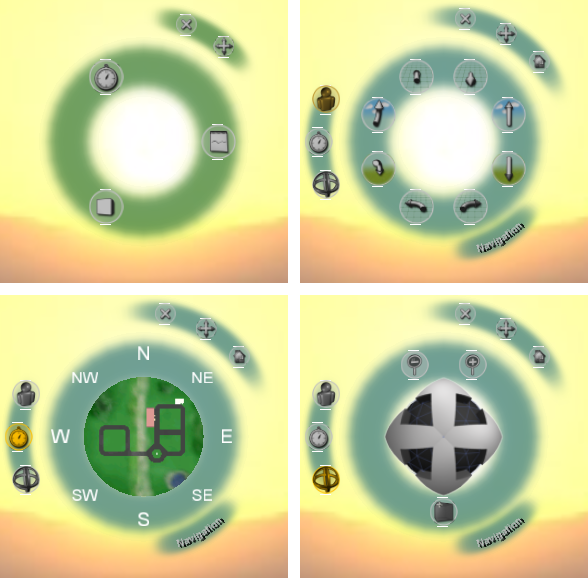
\includegraphics[scale=0.5]{gfx/main-nav-menus.png}
	\caption{Main menu and all 3 navigation menu modes}
	\label{fig:main-nav-menus}
\end{figure}


\subsection{First Person Mode}

This navigation mode is centered on the current point of view and works by triggering the displayed gates.
It features 8 gates: 4 direction displacement gates and 4 rotation gates.
To stop the movement/rotation one can either trigger the gate again, effectively disabling the ongoing action
or by triggering a different gate action.

The choice for this mode's layout suffered several evolutions.
At early stages opposing directions where placed at opposite sides of the ring but this
made correction by triggering the opposite action difficult, so opposing actions are now close together.
In this mode a restriction of one enabled action at a time is imposed to keep the handling easy for novice users.

There are gates for moving forward/backwards, up/down, pitch up/down and yaw up/down
\footnote{The verbs pitch and yaw come from flight semantics: to pitch is to look up/downwards; to yaw is to turn relatively to the ground plane.}.



\subsection{Compass Mode}

The compass mode was thought out for searching tasks. It allows the user to move along the ground plane and turn around it.
The compass navigation mode has 2 distinct areas:
the center circle displays a top-down view of the scene centered on the user;
the outer ring displays the main compass directions.
In order for one to move, a dragging movement must be performed inside the top-down view.
To reorient the user one must rotate the outer ring. The direction the user is facing can be read on the top part of the ring.

This mode could not be tested on multi-screen displays due to technical problems.
It was enthusiastically accepted on one-projector early tests.


\subsection{Examine Mode}

The examine mode allows the user to recenter attention on an object of the scene.
It features 3 gates and a center sphere.
The user must initially select the new center of attention by triggering the recenter gate,
finishing the stroke at the desired object/location.
Once the location is defined the remaining gates allow for zooming in and out the centered content
while the sphere allows for repositioning the user on the space around the object -- 
horizontal drags rotate horizontally, vertical moves vertically.

This mode is the most effective when performing shape modeling tasks.


\begin{figure}[ht]
	\centering
		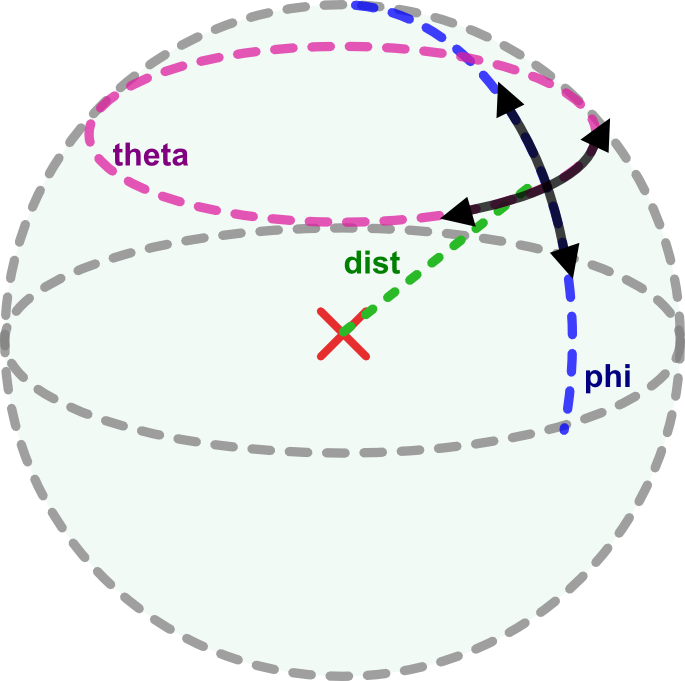
\includegraphics[scale=0.6]{gfx/virtual-sphere.png}
	\caption{Concept supporting examine mode}
	\label{fig:vsphere}
\end{figure}


\section{Content Creation}

The system's interface offers 3 families of shapes which can be instanced on the scene.
There are the primitives cube, cylinder and sphere; a set of previously generated shapes
and set of known building styles from which one can create buildings.
Primitives are the most versatile shapes since they support face and edge manipulation operations.
All shapes support simple transformations and cloning.

One uses building styles to create buildings on the scene. A library of generated shapes such as
people a trees serve as asserts to populate the scene with details and primitives can be instanced
as is or as building ground for custom shapes.

\begin{figure}[ht]
	\centering
		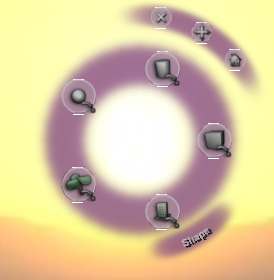
\includegraphics[scale=0.5]{gfx/shape.png}
	\caption{Shape menu}
	\label{fig:shape}
\end{figure}


\subsection{Shape Instancing}

The instancing of shapes works using the Apply-to-Scene concept described on section \ref{design:apply-to-scene}.
Every gate of this type has a small arrow running outwards as a hint to the user of this feature.
The user activates the gate of the desired shape and ends the stroke where he wants it to rest.



\subsection{Building Instancing}

%\TODO{ADD CALI TO BLOCKS, HERE AND TRIANGLE STROKE}
Once the building parameters have been gathered by the interface, as described on section \ref{design:building},
the building needs to be generated.
First the stroke is projected onto the construction plane and parsed by the shape recognizer as a rectangle.
The recognized rectangle dimensions serve as the blueprint which is extruded upwards for the measured height.
Then the building facades are generated according to the chosen style grammar and so is the ceiling.
The style grammar is fed each facade length and returns a set of spacings and facade elements that must be instanced
according to the rules defined in the style.
To minimize the facade attachments in memory, a map of loaded attachments is managed so only the first instance of any
attachment is loaded.


\subsection{Building Style Grammar}

\subsubsection{Grammar Structure}

The building style grammar defines building parameters such as
\textbf{floor-height}, \textbf{ceiling} parameters and \textbf{color-interval}s for the walls and ceiling.
It also defines a set of rules for the generation of the facade attachments that make up the final facades,
defined by the optional \textbf{front-facade} and the \textbf{facades} elements.

One can define the layout of a floor with the \textbf{layout} element, composed of 4 sections:
\textbf{left}, \textbf{center}, \textbf{right} and \textbf{other}.
Of these only the \textbf{other} section is required and the layout works by trying to fill the facade space with \textbf{center}, \textbf{left} and \textbf{right}s' contents if those are present, repeating \textbf{other}'s contents for filling the remaining space.

Inside these sections one can put any of the \textbf{us-element}s: \textbf{atom}, \textbf{group}, \textbf{sequence} and \textbf{random}.
An \textbf{atom} is the simplest \textbf{us-element}, having the attributes
\emph{type}, \emph{spacing} and \emph{height}.
The \emph{type} parameter defines which shape to instantiate on the facade,
\emph{spacing} how many length of the facade it will consume and
\emph{height} can be used to shift the shape upwards (to move a window, for instance).

The remaining \textbf{us-element}s allow combining \textbf{us-element}s.
A set of \textbf{us-element}s inside a \textbf{group} create all content on the same place and measure the longest of its children.
A set of \textbf{us-element}s inside a \textbf{sequence} create all children one after the other.
The \emph{random} \textbf{us-element} is similar to \textbf{group}, but has the attribute \emph{odds},
a set of comma separated ratios defining the probability of each child to be picked.

Several floors can share the same layout. To apply a layout to one or a set of floors, the floor-span element exists.
It can have either the \emph{at} attribute defined or both \emph{min} and \emph{max},
resulting in the application of the enclosed layout to all the floors in the interval.

One can also define a different facade style for the front facade with the element \textbf{front-facade}.
This is useful when one wants to apply columns and doors to one facade but not the remaining ones.


An example of a complete building style can be found on appendix \ref{residentialGrammar}. The resulting building is depicted on
figure .

\begin{figure}[ht]
	\centering
		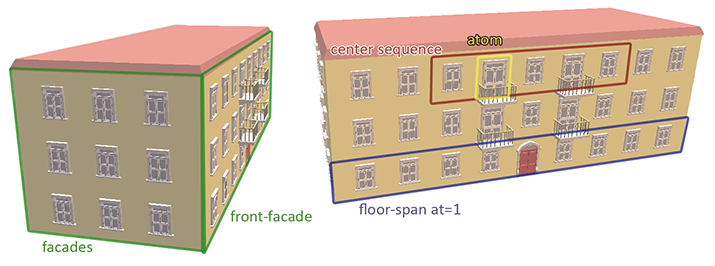
\includegraphics[width=\textwidth]{gfx/style.png}
	\caption{Resulting building of residential style. Several components are highlighted for comprehension.}
	\label{fig:style}
\end{figure}




\section{Content Editing}

All shapes in the system are made of 4-edged faces and all shapes are closed surfaces.
Operations such as the split by face loop rely on these properties.
Each shape computes each edge's neighboring faces (always 2)
and therefore each face's neighboring faces, forming an auxiliary structure called the edge map,
used for optimized queries for neighbors.

\TODO{summarize}

\subsection{Face Selection}

When a stroke finishes its start and ending points are projected onto the scene's available geometry.
If these 2 points lie on the same face of the same object that face is selected and the face contextual menu appears.

\begin{figure}[ht]
	\centering
		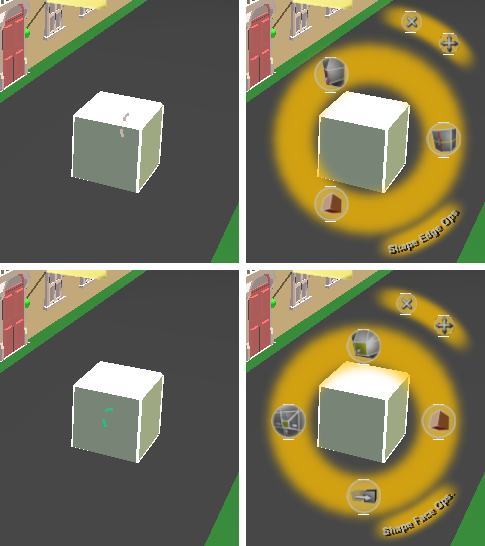
\includegraphics[scale=0.5]{gfx/face-edge-selection-imp.png}
	\caption{Edge and Face selection and their contextual menus}
	\label{fig:face-edge-selection-imp}
\end{figure}



\subsection{Edge Selection}

If the stroke start and ending points lie on different but neighboring faces of the same shape, the edge between
those faces is selected and the edge contextual menu appears.


\subsection{Determining and Selecting Directions}

In order to keep the interface simple and to minimize the number of steps to perform an operation, a set of directions
is estimated for edge and face selections -- these are believed to be the most frequently needed vectors for shape operations.
When an edge is selected the computed directions are the edge outwards normal and the directions from the edge along its neighboring faces.
When a face is selected the computed directions are the face normal along with the 4 directions from the center of the face
to each of its neighboring faces.

If an operation requires the user to select a direction from the user the computed directions are displayed centered on the selected aspect
and color coded. The interface relies on the user to keep drawing the stroke after the operation is triggered so the remaining of the stroke's direction serves to select the desired direction by approximation -- while the stroke is being drawn the operation is previewed by applying the currently most approximate vector direction to the shape. The length of the stroke can be also used from the provided information by using the stroke's direct length.

\begin{figure}[ht]
	\centering
		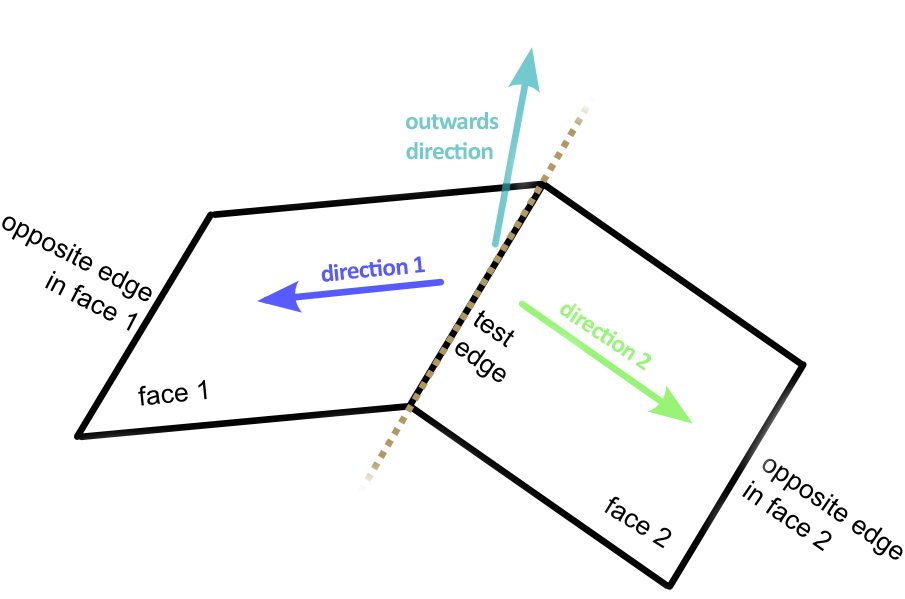
\includegraphics[scale=0.6]{gfx/face-dirs.png}
	\caption{Face directions}
	\label{fig:face-dirs}
\end{figure}


\begin{figure}[ht]
	\centering
		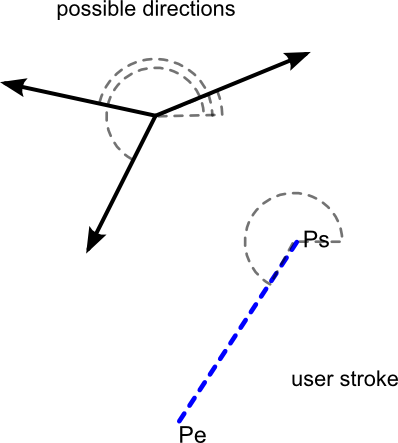
\includegraphics[scale=0.6]{gfx/election.png}
	\caption{Direction selection}
	\label{fig:election}
\end{figure}




\subsection{Shape Operations}

\begin{figure}[ht]
	\centering
		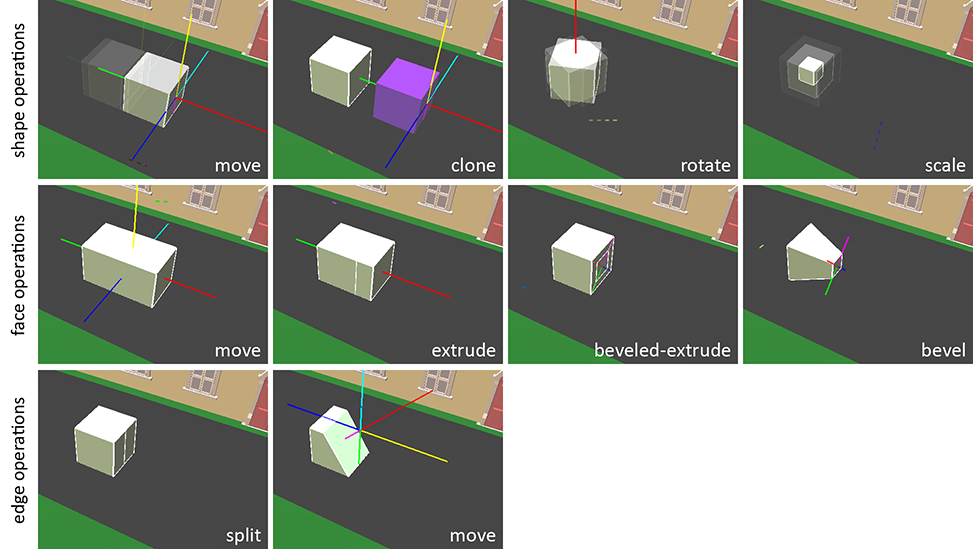
\includegraphics[width=\textwidth]{gfx/ops.png}
	\caption{Shape operation example applications}
	\label{fig:ops}
\end{figure}


By selecting a face the following operations can be performed:
\begin{itemize}
	\item \textbf{extrude face} - Extrude generates 4 additional faces, getting the direction from the selected face's normal and the displacement from stroke length.
	\item	\textbf{bevel face} - Bevel moves the face vertices, getting distance from stroke length.
	\item	\textbf{extrude \& bevel} - This is a compound operation of zero length extrude followed by bevel. It exists for convenience to aid in the creation of holes for features such as windows or chimneys.
	\item	\textbf{move face} - Move face displaces the face vertices, getting the direction from the selected face's normal and 4 computed directions.
	\item	\textbf{move coplanar faces} - This operation works as the previous one but the neighboring faces having an angle with the selected one smaller than the threshold are also affected by the movement.
\end{itemize}

By selecting an edge the following operations can be performed:
\begin{itemize}
	\item \textbf{move edge} - Moves the edge vertices along one of the directions: edge normal and neighboring faces, obtaining the displacement from stroke length.
	\item	\textbf{split at face loop} - The crossed edge defines a direction. All faces on that face loop are split in the middle, creating additional geometry. This operation has instant application as it doesn't require additional data.
\end{itemize}

On both edge and face context menus there's an option to \textbf{toggle} the visibility of the \textbf{shape edges}.

All shapes have a stack of memento objects for supporting the undo operation, also available on both menus.
The memento design pattern states that an auxiliary object - the memento object - decorates the state of the key object structures so they
can be restored if backup is needed.


\section{Reviewing}

Notes can be created on the scene. A menu exists featuring a large area at the center where strokes can be drawn as if writing on paper.
A rubber option allows wiping the note contents. Once the note is written it can be attached to any scene object by using the
apply-to-scene concept. Notes are real 3D entities and can be hidden or edited by performing a closed stroke around them.

\begin{figure}[ht]
	\centering
		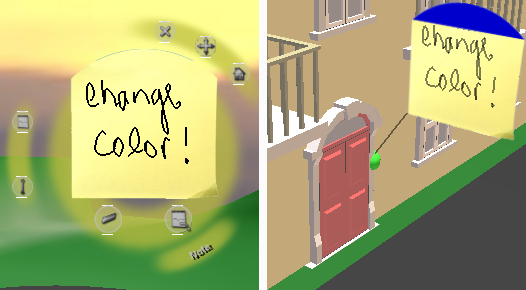
\includegraphics[scale=0.5]{gfx/note.png}
	\caption{Creating a note and the result attached to a door}
	\label{fig:note}
\end{figure}


\section{Proposed Work Flow}

Shapes can be loaded or saved to XML and the simple descriptive format can be easily supported by 3D modelers.
For the purposes of the generation of terrains, library objects and facade attachments the Blender 3D modeling package
was used and an exporting plug-in developed.

\subsection{Scenario Creation}

The system is a prototype tool so not much emphasis was put into the importing of content.
Even so, different scenarios could be created.
The height data from a terrain patch can be represented by either:
\begin{itemize}
	\item an height map - a gray-scale matrix with highest values represented by brighter colors.
	\item a topographic map - a discrete set of contour lines uniting points with the same altitude.
\end{itemize}

With any of these data a 3D mesh can be generated - by vertex shifting a regular mesh for height maps or applying
a Delaunay triangulation to the contour lines.
With additional satellite imagery the terrain appearance could also be approximated by vertex coloring or texture projection application.


\subsection{Building Style Creation}

New attachment shapes could be created using Urban Sketcher itself or an auxiliary 3D modeler.
Creating a building style is a matter of editing the style grammar, defining ceiling type, colors, floor height and most of all
the layout for the building floors using existing and/or newly created attachments.


\TODO{UPDATED WORK FLOW DIAGRAM}

\TODO{example stages}

